\Chapter{Related Work}\label{chapter:related}

In this chapter, I provide a comprehensive review of existing
approaches relevant to multi-view image generation.

The chapter begins by introducing the fundamental task of Novel View
Synthesis (NVS) and its significance. We then delve into traditional
3D reconstruction techniques (Section \ref{sec:3d-reconstruction})
and their inherent limitations, particularly for sparse-input
scenarios, which motivates the exploration of generative methods.
Subsequently, the discussion shifts to the foundational principles of
Deep Generative Models for Image Synthesis, with a focus on diffusion
models (Section \ref{sec:text-to-image}).

Building on this, we explore various methods for Conditioning
Diffusion Models for Enhanced Control and New Tasks (Section
\ref{sec:conditioning-diffusion}), including the crucial role of
camera parameter encoding and the concept of lightweight adaptation
through adapters.

The core of the chapter then examines state-of-the-art
Diffusion-based Multi-View Image Generation techniques (Section
\ref{sec:multi-view-diffusion}), covering both single reference image
novel view synthesis and architectures for coherent multi-view
generation, including specialized multi-view adapters.
%  Finally, the chapter will conclude with a summary of the discussed
% methods and highlight identified research gaps that this thesis
% aims to address.

\section{Traditional 3D Reconstruction Approaches}\label{sec:3d-reconstruction}

Simultaneous Localization and Mapping (SLAM) is a fundamental concept
in the field of computer vision and robotics. It refers to the
process of simultaneously estimating the camera's position and
orientation in a 3D environment while mapping the environment itself.
Originally, SLAM was used to track the position of a robot in a 3D
space, but it has since been applied to a wide range of problems,
including augmented reality, medical applications and novel view
synthesis.

SLAM works by processing sensor data in real-time to create a map of the unknown environment while simultaneously tracking the position of the sensor within that map. This process typically involves several key steps:
\begin{enumerate}
  \item \textbf{Feature Detection}: Identifying distinctive points or features in the environment from sensor data
  \item \textbf{Data Association}: Matching observed features with previously mapped features
  \item \textbf{State Estimation}: Updating the estimated pose of the camera and the map of the environment
  \item \textbf{Loop Closure}: Recognizing when the sensor has returned to a previously visited location and adjusting the map accordingly to reduce accumulated errors
\end{enumerate}

To address these requirements, researchers have
concentrated on creating techniques for machines to independently
build ever more precise scene representations. This integration of
robotics, computer vision, sensor technology, and recent advancements
in artificial intelligence has shaped this field.

Typically, SLAM techniques use a combination of data sources, such as
images, laser range scans, sonars and GPS to effectively map an environment.
In this work I will focus on the use of images for 3D reconstruction.

\subsection{Structure from Motion Pipeline}

One of the most popular methods for 3D reconstruction from images is
COLMAP \cite{colmap}. COLMAP is a general-purpose
structure-from-motion (SfM) \cite{multipleviewgeometry} system that
can automatically reconstruct 3D scenes from a collection of images.
It is a popular choice for 3D reconstruction due to its accuracy,
speed, and ease of use.

\begin{figure}[h]
  \centering
  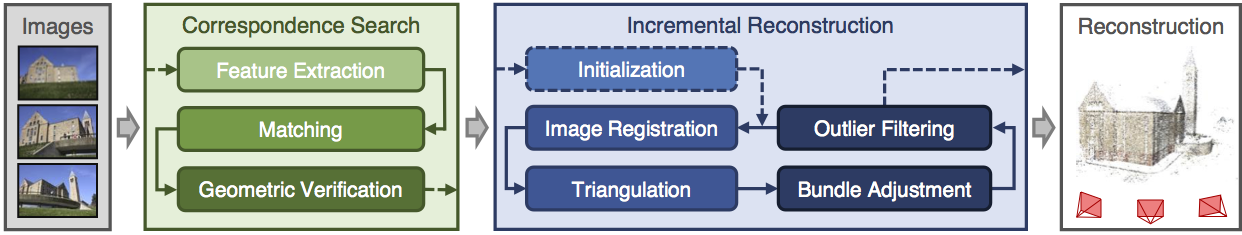
\includegraphics[width=0.9\textwidth]{images/related-work/COLMAP.png}
  \caption{COLMAP pipeline}
  \label{fig:colmap-pipeline}
  % https://colmap.github.io/tutorial.html
\end{figure}

Structure from Motion works in two main steps [Figure
\ref{fig:colmap-pipeline}]:
\begin{enumerate}
  \item \textbf{Correspondence Search}: Identify the unique landmarks
    (features) in all of the images and match the same landmarks across images.
  \item \textbf{Incremental Reconstruction}: Estimates the camera
    poses and triangulates 3D points through an iterative process.
\end{enumerate}

First step of correspondence search is feature extraction. COLMAP
uses SIFT \cite{sift} and ORB \cite{orb} methods to extract features
from images. Scale-invariant feature transform (SIFT) is a method for
detecting keypoints that contrast with their surroundings and
describing the local image content around them. It is invariant to
rotation and scale, making it robust for matching features across images taken from different viewpoints and distances. Oriented FAST and Rotated BRIEF (ORB) is a more
computationally efficient alternative to SIFT, combining a high-speed
FAST detector with optimized descriptors for rotation invariance,
offering comparable matching performance with significantly reduced computational requirements.

\begin{figure}[h]
  \centering
  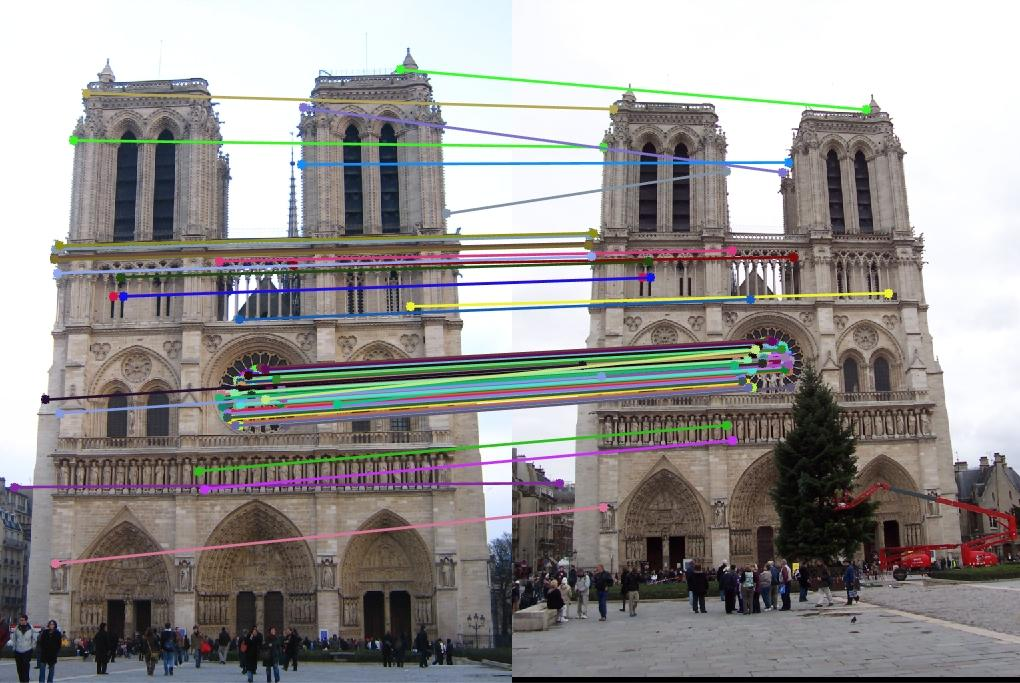
\includegraphics[width=0.7\textwidth]{images/related-work/feature-matching.jpg}
  \caption{Feature matching result}
  \label{fig:matching-features}
  % https://blog.roboflow.com/image-matching/
\end{figure}

Second step is matching features across images. Feature matching is a
process of finding the best matches of features across the images.
COLMAP uses a variant of the FLANN \cite{flann} library to find the
best matches for each feature. FLANN is a library for performing fast
approximate nearest neighbor searches in high dimensional spaces.
Feature matching is visualized in Figure \ref{fig:matching-features}.

Then the geometric verification step uses the prior knowledge about
the camera model and motion to remove outliers, preparing the
verified feature matches for the subsequent Incremental Reconstruction phase.

When it comes to Incremental Reconstruction, the process is as follows:
\begin{enumerate}
  \item \textbf{Camera Pose Estimation}: Estimate the camera location
    and direction in 3D space for each image.
  \item \textbf{Triangulation}: Triangulate 3D points of the observed
    objects from the camera poses and matched features.
  \item \textbf{Bundle Adjustment}: Refine the camera poses and 3D
    points to minimize the reprojection error.
\end{enumerate}

\begin{figure}[h]
  \centering
  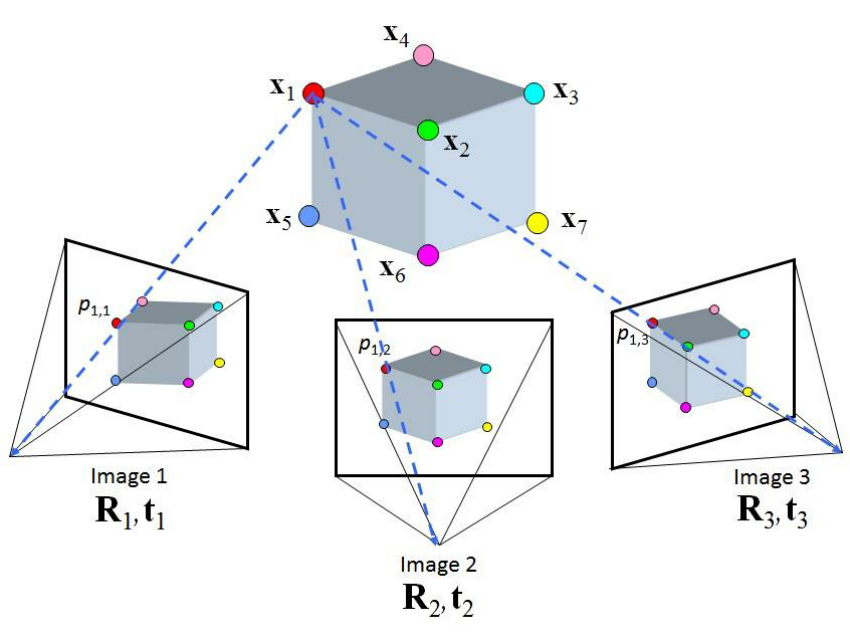
\includegraphics[width=0.5\textwidth]{images/related-work/Structure-from-Motion-SfM-process-is-illustrated-The-structure-in-the.png}
  \caption{Camera pose estimation}
  \label{fig:camera-pose-estimation}
  % https://www.researchgate.net/figure/Structure-from-Motion-SfM-process-is-illustrated-The-structure-in-the_fig2_269327935
\end{figure}

The camera pose estimation (visualized in Figure
\ref{fig:camera-pose-estimation}) starts with an initialization step,
where the initial pair of images and matched features between them
are used to estimate the camera pose. Then, the algorithm proceeds to
the loop (Figure \ref{fig:colmap-pipeline}), where the next image is
registered to the reconstruction and the camera pose is estimated
again (triangulation step). After that the bundle adjustment step is
performed to refine the camera poses and 3D points to be consistent
with the entire dataset with images of a given scene. This
optimization process typically uses the Levenberg-Marquardt algorithm
to minimize reprojection error. This process is repeated for each
subsequent batch of images, updating the camera poses and 3D points.

\subsection{Methods for 3D Reconstruction}

The field of 3D reconstruction encompasses various approaches beyond the basic Structure from Motion pipeline. These methods can be broadly categorized into two groups: sparse reconstruction (like SfM) and dense reconstruction methods.

\subsubsection{Dense Reconstruction Methods}

While SfM provides camera poses and a sparse point cloud, dense reconstruction methods aim to create a complete 3D model with detailed surface information. Notable methods include:

\begin{enumerate}
  \item \textbf{Multi-View Stereo (MVS)}: After obtaining camera poses through SfM, MVS algorithms like PMVS \cite{pmvs} generate dense point clouds by matching pixels across multiple images.

  \item \textbf{Depth Map Fusion}: Methods such as COLMAP's MVS pipeline estimate per-image depth maps and then fuse them into a consistent 3D model.

  \item \textbf{Neural Radiance Fields (NeRF)} \cite{nerf}: A more recent approach that represents scenes as continuous 5D functions (spatial location and viewing direction) encoded in neural networks. NeRF takes camera poses from SfM as input and uses ray tracing to synthesize novel views with remarkable detail and view consistency.
\end{enumerate}

\subsubsection{Learning-based Reconstruction}

Recent approaches leverage deep learning for 3D reconstruction, often using SfM-derived data for supervision or initialization:

\begin{enumerate}
  \item \textbf{Learned MVS}: Methods like MVSNet \cite{mvsnet} use convolutional neural networks to learn the depth estimation process directly from images and camera parameters.

  \item \textbf{Single-view Reconstruction}: Networks like Mesh R-CNN \cite{meshrcnn} can estimate 3D structure from a single image by leveraging prior knowledge learned from large datasets.
\end{enumerate}

\subsection{Limitations of 3D Reconstruction}

Structure from Motion is a powerful tool for 3D reconstruction, demonstrating high effectiveness across a variety of scenarios. However, it encounters significant challenges. These include dealing with textureless surfaces, reflective materials, and the computational complexity of processing high-resolution images. Most importantly in the context of this thesis, it struggles with sparse input scenarios, such as those involving a single image or only a few images.

Traditional 3D reconstruction methods like SfM and MVS typically require a dense collection of images with sufficient overlap to establish accurate feature correspondences and camera pose estimations. When faced with limited input views—particularly in the extreme case of a single image—these methods often fail to generate complete and accurate 3D representations. The quality of reconstruction degrades significantly due to:

\begin{enumerate}
  \item \textbf{Geometric ambiguity}: A single image or sparse set of images provides incomplete information about occluded regions and depth, leading to ambiguous geometry.

  \item \textbf{Feature matching limitations}: Fewer images means fewer opportunities to establish reliable feature correspondences across different viewpoints.

  \item \textbf{Inability to triangulate}: Robust triangulation requires features to be visible from multiple viewpoints, which is not possible with very limited inputs.

  \item \textbf{View-dependent effects}: Materials with specular reflections or varying appearance based on viewpoint cannot be accurately modeled without multiple observations.
\end{enumerate}

These limitations have motivated the development of generative approaches to novel view synthesis, particularly using diffusion models trained on large datasets of rendered images of 3D models. Instead of explicitly reconstructing geometry, these methods leverage the power of deep learning to hallucinate plausible views from unseen perspectives.

\begin{figure}[h]
  \centering
  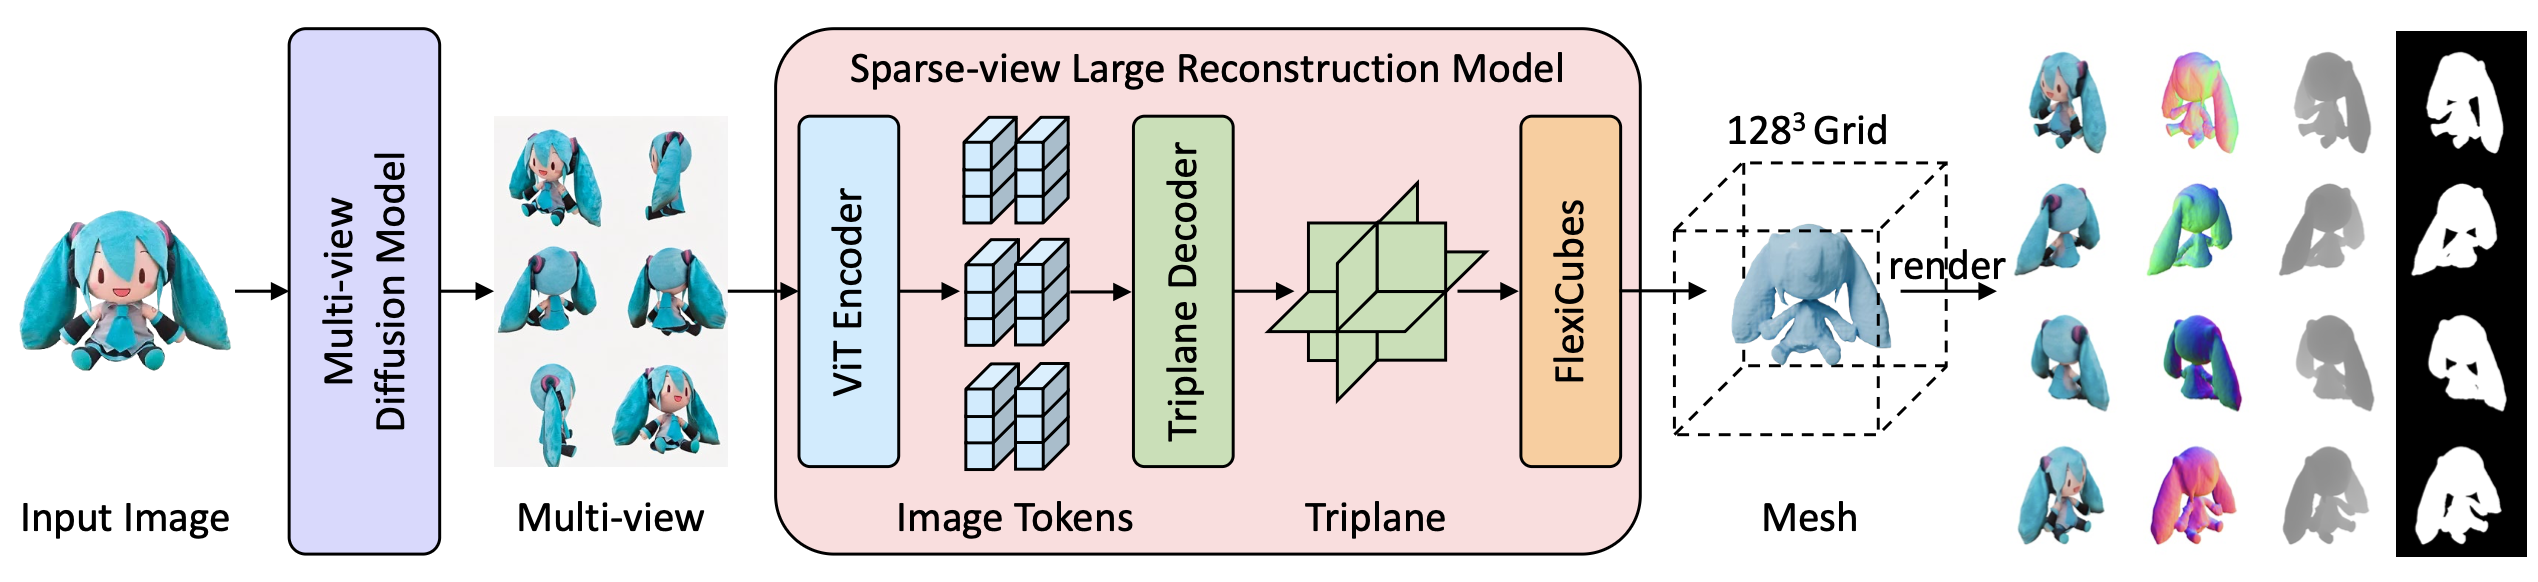
\includegraphics[width=\textwidth]{images/related-work/instantmesh.png}
  \caption{InstantMesh}
  \label{fig:instantmesh}
\end{figure}

Modern approaches of 3D object generation, such as InstantMesh \cite{instantmesh}, leverage these diffusion models to generate multiple consistent views of an object from minimal input (a single image or even a text prompt). This novel view synthesis is the first step in a pipeline \ref{fig:instantmesh} that can be used to create a 3D model of the object, and it is this particular step that forms the central focus of this thesis.

\section{Deep Generative Models for Image Synthesis}\label{sec:text-to-image}

The development of deep learning methods has led to remarkable progress in generative modeling, enabling the synthesis of highly realistic and diverse images. Among the various approaches, Generative Adversarial Networks (GANs), Variational Autoencoders (VAEs), and Diffusion Models have emerged as the most prominent. While GANs and VAEs have laid significant groundwork and continue to be influential, this section will primarily focus on diffusion models, given their state-of-the-art performance in image quality and controllability, and their direct relevance to the multi-view synthesis tasks explored in this thesis.

\subsection{Generative Adversarial Networks (GANs) and Variational Autoencoders (VAEs)}

Generative Adversarial Networks (GANs) \cite{gan} consist of two neural networks, a generator and a discriminator, trained in a competitive setting. The generator aims to produce realistic images, while the discriminator tries to distinguish between real images from the training dataset and fake images produced by the generator. Through this adversarial process, the generator learns to create increasingly plausible images. GANs are known for generating sharp images but often suffer from training instability.

Variational Autoencoders (VAEs) \cite{vae} are another class of generative models that learn a probabilistic mapping from a high-dimensional data space (e.g., images) to a lower-dimensional latent space, and then back to the data space. A VAE consists of an encoder that compresses the input data into a latent representation (typically a mean and variance defining a Gaussian distribution) and a decoder that reconstructs the data from samples drawn from this latent distribution. They are trained to maximize the evidence lower bound (ELBO), which involves a reconstruction loss and a regularization term (KL divergence) that encourages the latent space to be smooth and well-behaved. VAEs generally offer more stable training than GANs and can learn a meaningful latent space, but often produce slightly blurrier images. VAEs play a crucial role in the architecture of Latent Diffusion Models.

\subsection{Diffusion Models}
Diffusion models have recently become the dominant paradigm in high-fidelity image generation. They are inspired by non-equilibrium thermodynamics, specifically diffusion processes.

\subsubsection{Core Concept: The Diffusion Process}
The core idea behind diffusion models involves two processes: a forward (or diffusion) process and a reverse (or denoising) process.
In the \textbf{forward process}, a known image $x_0$ from the dataset is gradually perturbed by adding small amounts of Gaussian noise over a sequence of $T$ steps. This process progressively corrupts the image until, at step $T$, it becomes indistinguishable from pure isotropic Gaussian noise. The parameters of this noising process are fixed.

The \textbf{reverse process} aims to learn to reverse this noising. Starting from pure noise (equivalent to $x_T$), a neural network is trained to gradually denoise the signal, step-by-step, eventually producing a realistic image (an approximation of $x_0$). This learned denoising process is what allows the model to generate new images. Figure \ref{fig:diffusion-process} illustrates this concept.

\begin{figure}[h]
  \centering
  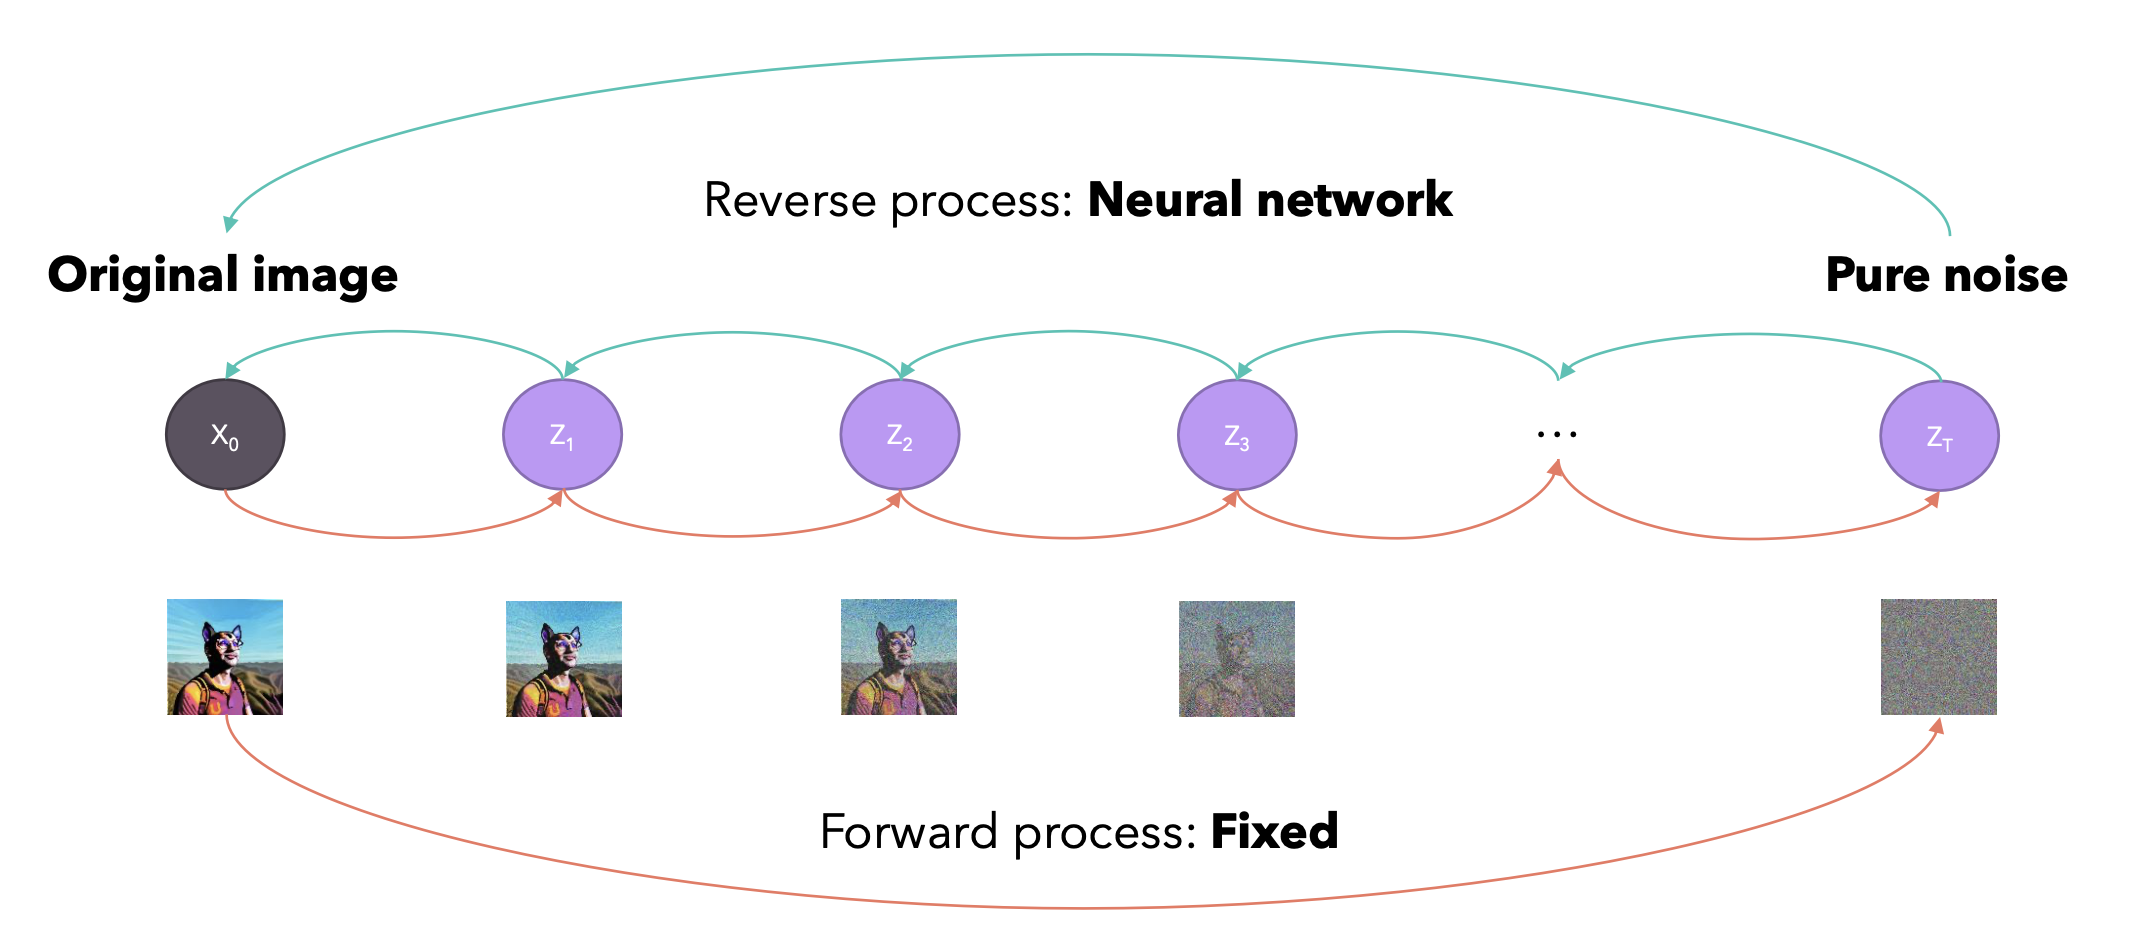
\includegraphics[width=0.8\textwidth]{images/related-work/diffusion-process.png}
  \caption{The forward (noising) and reverse (denoising/generation) stages of a diffusion model. The forward process gradually adds noise to an image until it becomes pure noise. The reverse process learned by a neural net to denoise, step-by-step, to generate an image from noise.}
  \label{fig:diffusion-process}
\end{figure}

\subsubsection{The U-Net Architecture}
The neural network responsible for predicting the noise (or the denoised image) at each step in the reverse process is typically a U-Net architecture \cite{unet}. The U-Net, originally developed for biomedical image segmentation, features an encoder-decoder structure with skip (residual) connections. The encoder path progressively downsamples the input, capturing contextual information, while the decoder path progressively upsamples, localizing information. The skip connections concatenate features from the encoder to corresponding layers in the decoder, allowing the network to combine high-level semantic information with low-level detail, which is crucial for accurately predicting the noise and preserving image fidelity during the denoising steps.

\subsubsection{Training Objective and Loss Function}
The training objective of the diffusion model is to learn the conditional probability distribution $p_\theta(x_{t-1}|x_t)$, which represents the probability of the previous, less noisy state $x_{t-1}$ given the current noisy state $x_t$. In practice, this is often simplified to training the U-Net to predict the noise $\epsilon$ that was added to an image $x_0$ to produce $x_t$ at a given timestep $t$. The loss function is typically the Mean Squared Error (MSE) between the true added noise $\epsilon$ and the noise $\epsilon_\theta(x_t, t)$ predicted by the U-Net:
\[ L = \mathbb{E}_{t \sim [1, T], x_0 \sim q(x_0), \epsilon \sim \mathcal{N}(0, I)} [\|\epsilon - \epsilon_\theta(x_t, t)\|^2] \]
where $x_t = \sqrt{\bar{\alpha}_t}x_0 + \sqrt{1-\bar{\alpha}_t}\epsilon$, and $\bar{\alpha}_t$ are parameters from the noise schedule.

\subsubsection{Conditional Generation: Text-to-Image Synthesis}
To guide the image generation process, diffusion models can be conditioned on various inputs, most notably text prompts. This is the foundation of text-to-image synthesis.
A crucial component for text conditioning is a powerful text encoder that can convert textual descriptions into rich numerical representations (embeddings). Contrastive Language-Image Pre-training (CLIP) \cite{clip} is widely used for this purpose. CLIP is trained on a massive dataset of image-text pairs to learn a shared embedding space where semantically similar images and texts are close together.

The text embeddings from CLIP are then integrated into the U-Net, typically using cross-attention mechanisms. In these layers, the image representation at an intermediate layer of the U-Net queries the text embedding, allowing the model to align parts of the image with relevant words or phrases in the prompt. This enables fine-grained control over the generated image content based on the textual input.

\subsection{Latent Diffusion Models (LDMs)}\label{ssec:ldm}
While standard diffusion models operate directly in the pixel space of images, this can be computationally very expensive, especially for high-resolution images, as the U-Net needs to process large tensors. Latent Diffusion Models (LDMs) \cite{stablediffusion}, such as Stable Diffusion, address this challenge by performing the diffusion and denoising process in a lower-dimensional latent space.

LDMs employ a pre-trained autoencoder, typically a VAE. The VAE's encoder first compresses a high-resolution image from pixel space into a compact latent representation. The diffusion process (both forward and reverse) then occurs entirely within this latent space. Once the reverse denoising process generates a target latent representation from noise, the VAE's decoder maps this latent representation back into the high-resolution pixel space to produce the final image. Figure \ref{fig:ldm-architecture} depicts the architecture of an LDM.

\begin{figure}[h]
  \centering
  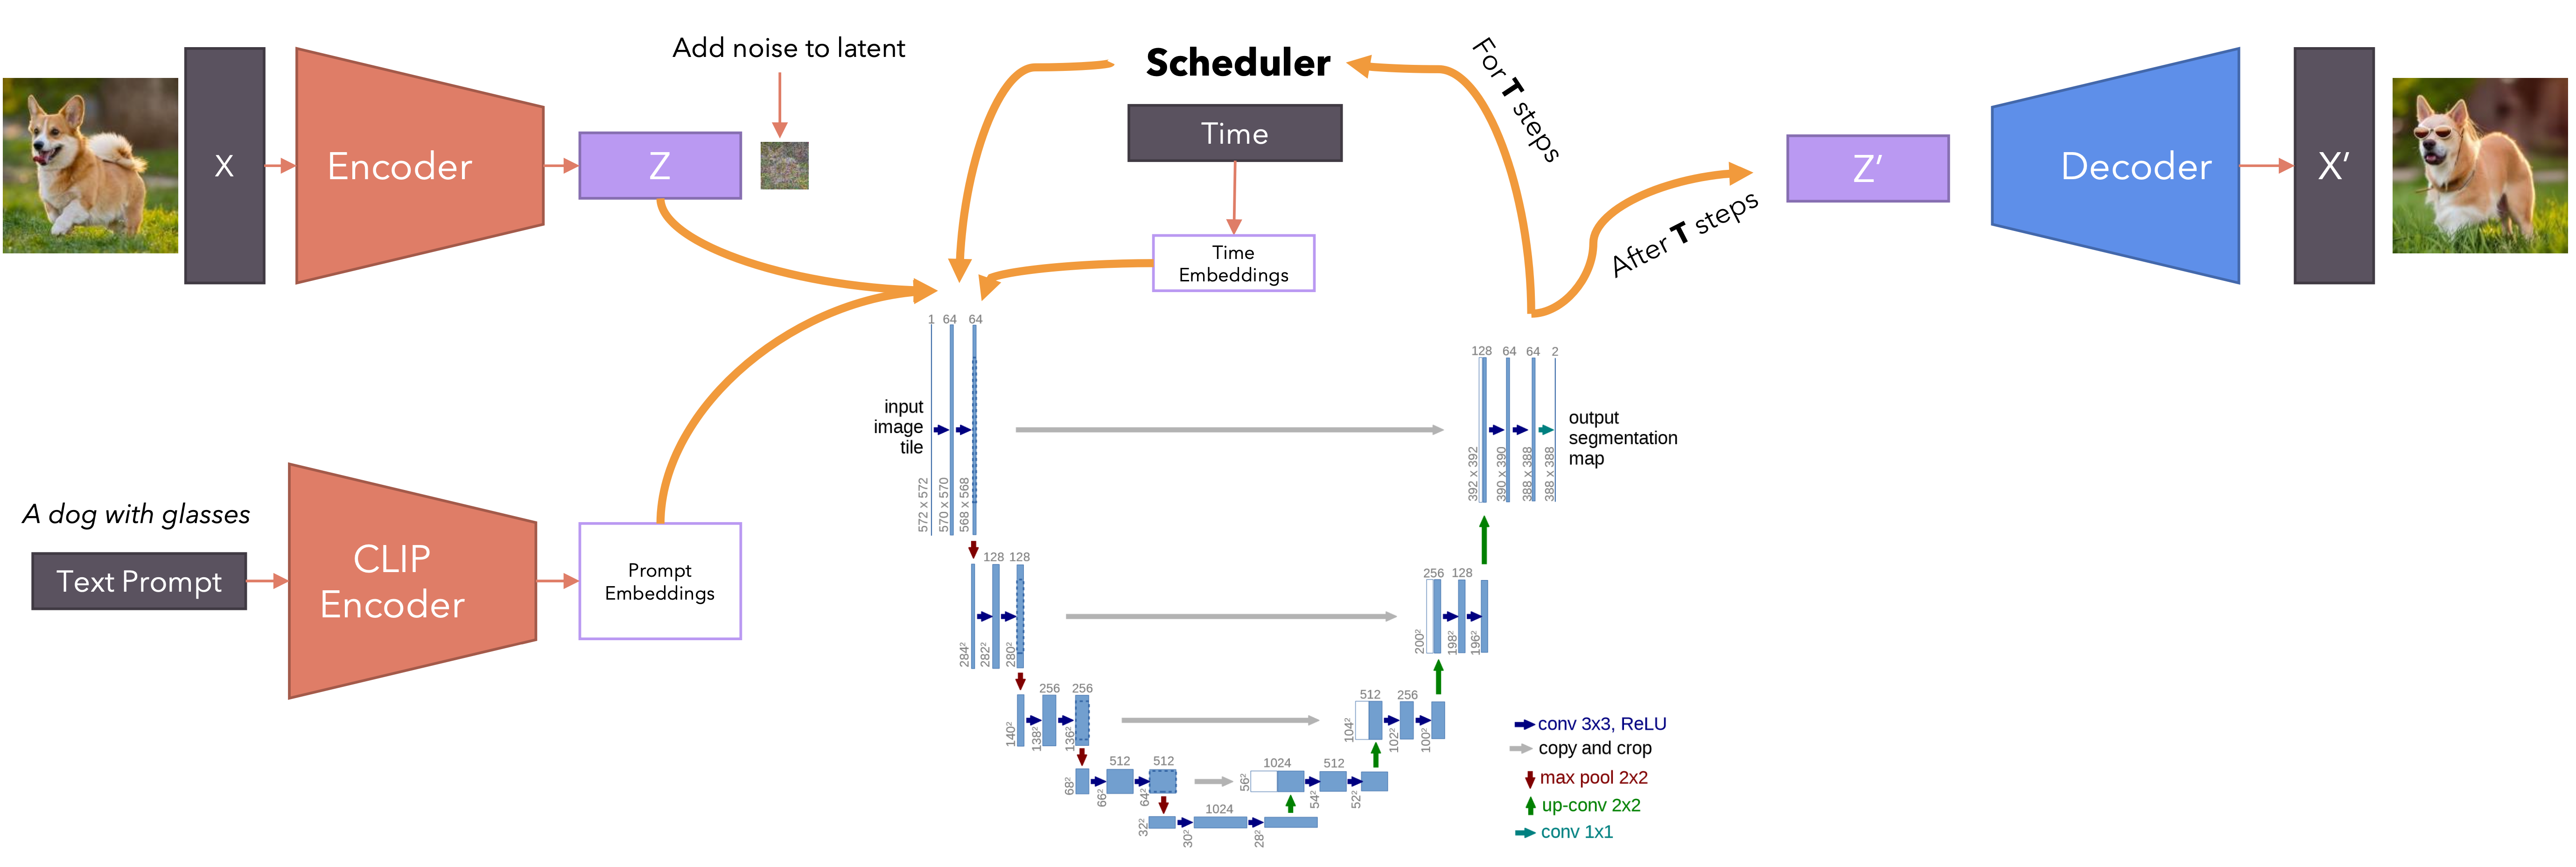
\includegraphics[width=\textwidth]{images/related-work/LDM-detailed.png}
  \caption{Architecture of a Latent Diffusion Model (LDM). An image is first encoded into a latent space by a VAE encoder. The diffusion process (noising and denoising via U-Net) occurs in this latent space. The generated latent is then decoded back to pixel space by the VAE decoder. Conditioning, such as text embeddings from CLIP, is incorporated into the U-Net.}
  \label{fig:ldm-architecture}
\end{figure}

By working in a compressed latent space, LDMs significantly reduce the computational burden during training and inference compared to pixel-space diffusion models. This makes it feasible to train powerful models on massive datasets and generate high-resolution images more efficiently, without a substantial loss in quality. The VAE ensures that the latent space is perceptually equivalent to the pixel space, and the diffusion model learns to generate high-quality latents within this space.

\section{Conditioning Diffusion Models for Enhanced Control and New Tasks}\label{sec:conditioning-diffusion}

While textual prompts provide a powerful and intuitive way to guide diffusion models, the generation process can be conditioned on a much wider array of signals. This opens up possibilities for more fine-grained control over the output and enables new applications beyond text-to-image synthesis. This section explores several advanced conditioning mechanisms, focusing on image-based conditioning for detailed content and style control, and specialized techniques for incorporating geometric information, such as camera parameters, to enrich 2D diffusion models with 3D awareness.

\subsection{Image-based Conditioning for Fine-Grained Control}
Conditioning on reference images allows for precise control over spatial layout, object appearance, color consistency, or artistic style, going beyond what is often achievable with text alone.

\subsubsection{ControlNet}
ControlNet \cite{controlnet} introduces a method to add diverse spatial conditioning to pre-trained text-to-image diffusion models. Instead of fine-tuning the original large model, ControlNet involves training smaller, task-specific auxiliary networks that are attached to the frozen U-Net backbone of the diffusion model, typically to its encoder blocks. These auxiliary networks take an input conditioning image (e.g., an edge map, human pose skeleton, depth map, or segmentation map) and produce feature maps that are then added to the corresponding features of the main U-Net. This approach allows the pre-trained model to be guided by the spatial information in the conditioning image while retaining its vast generative capabilities learned from large datasets. The original U-Net weights are locked, making ControlNet modules efficient to train and portable. Figure \ref{fig:controlnet-overview} provides a conceptual overview.

\begin{figure}[ht]
  \centering
  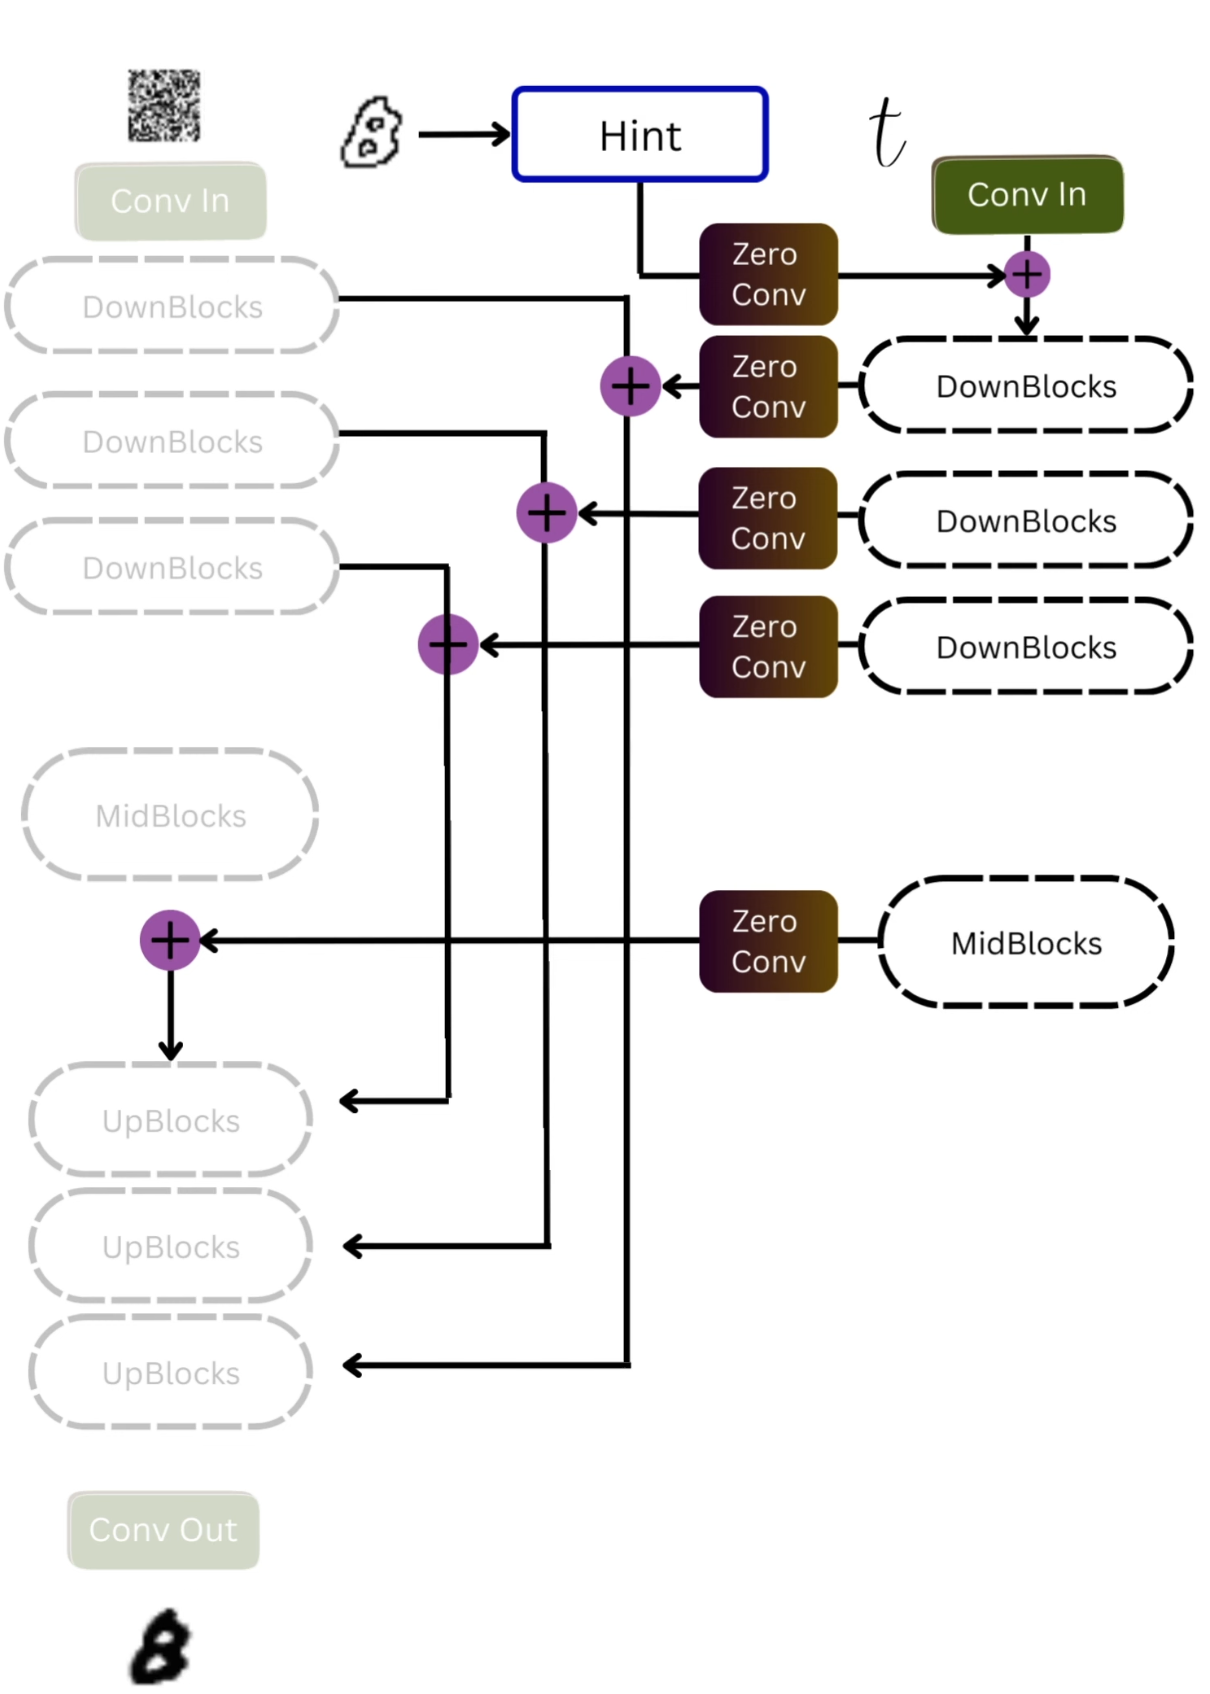
\includegraphics[width=0.4\textwidth]{images/related-work/controlnet.png}
  \caption{Conceptual overview of ControlNet, showing how an additional control module processes an input condition (e.g., edges, pose) and injects guidance into a pre-trained diffusion model. (Adapted from Zhang et al. \cite{controlnet})}
  \label{fig:controlnet-overview}
\end{figure}

\subsubsection{IP-Adapter}
IP-Adapter (Image Prompt Adapter) \cite{ipadapter} offers an effective way to condition diffusion models using an image prompt, allowing the model to generate images that align with the content or style of the reference image. It achieves this by introducing a lightweight adapter module that can be plugged into a pre-trained text-to-image model. The core idea is to decouple the cross-attention mechanisms used for text and image features. Image features, extracted by an image encoder (like CLIP \cite{clip} image encoder), are fed into new cross-attention layers that work in parallel with the original text cross-attention layers. This allows the model to draw information from both text and image prompts simultaneously or prioritize one over the other. IP-Adapter is efficient as it avoids fine-tuning the large base model and only trains the adapter parameters, making it a versatile tool for tasks like style transfer or subject-driven generation. Figure \ref{fig:ipadapter-concept} illustrates this concept.

\begin{figure}[h]
  \centering
  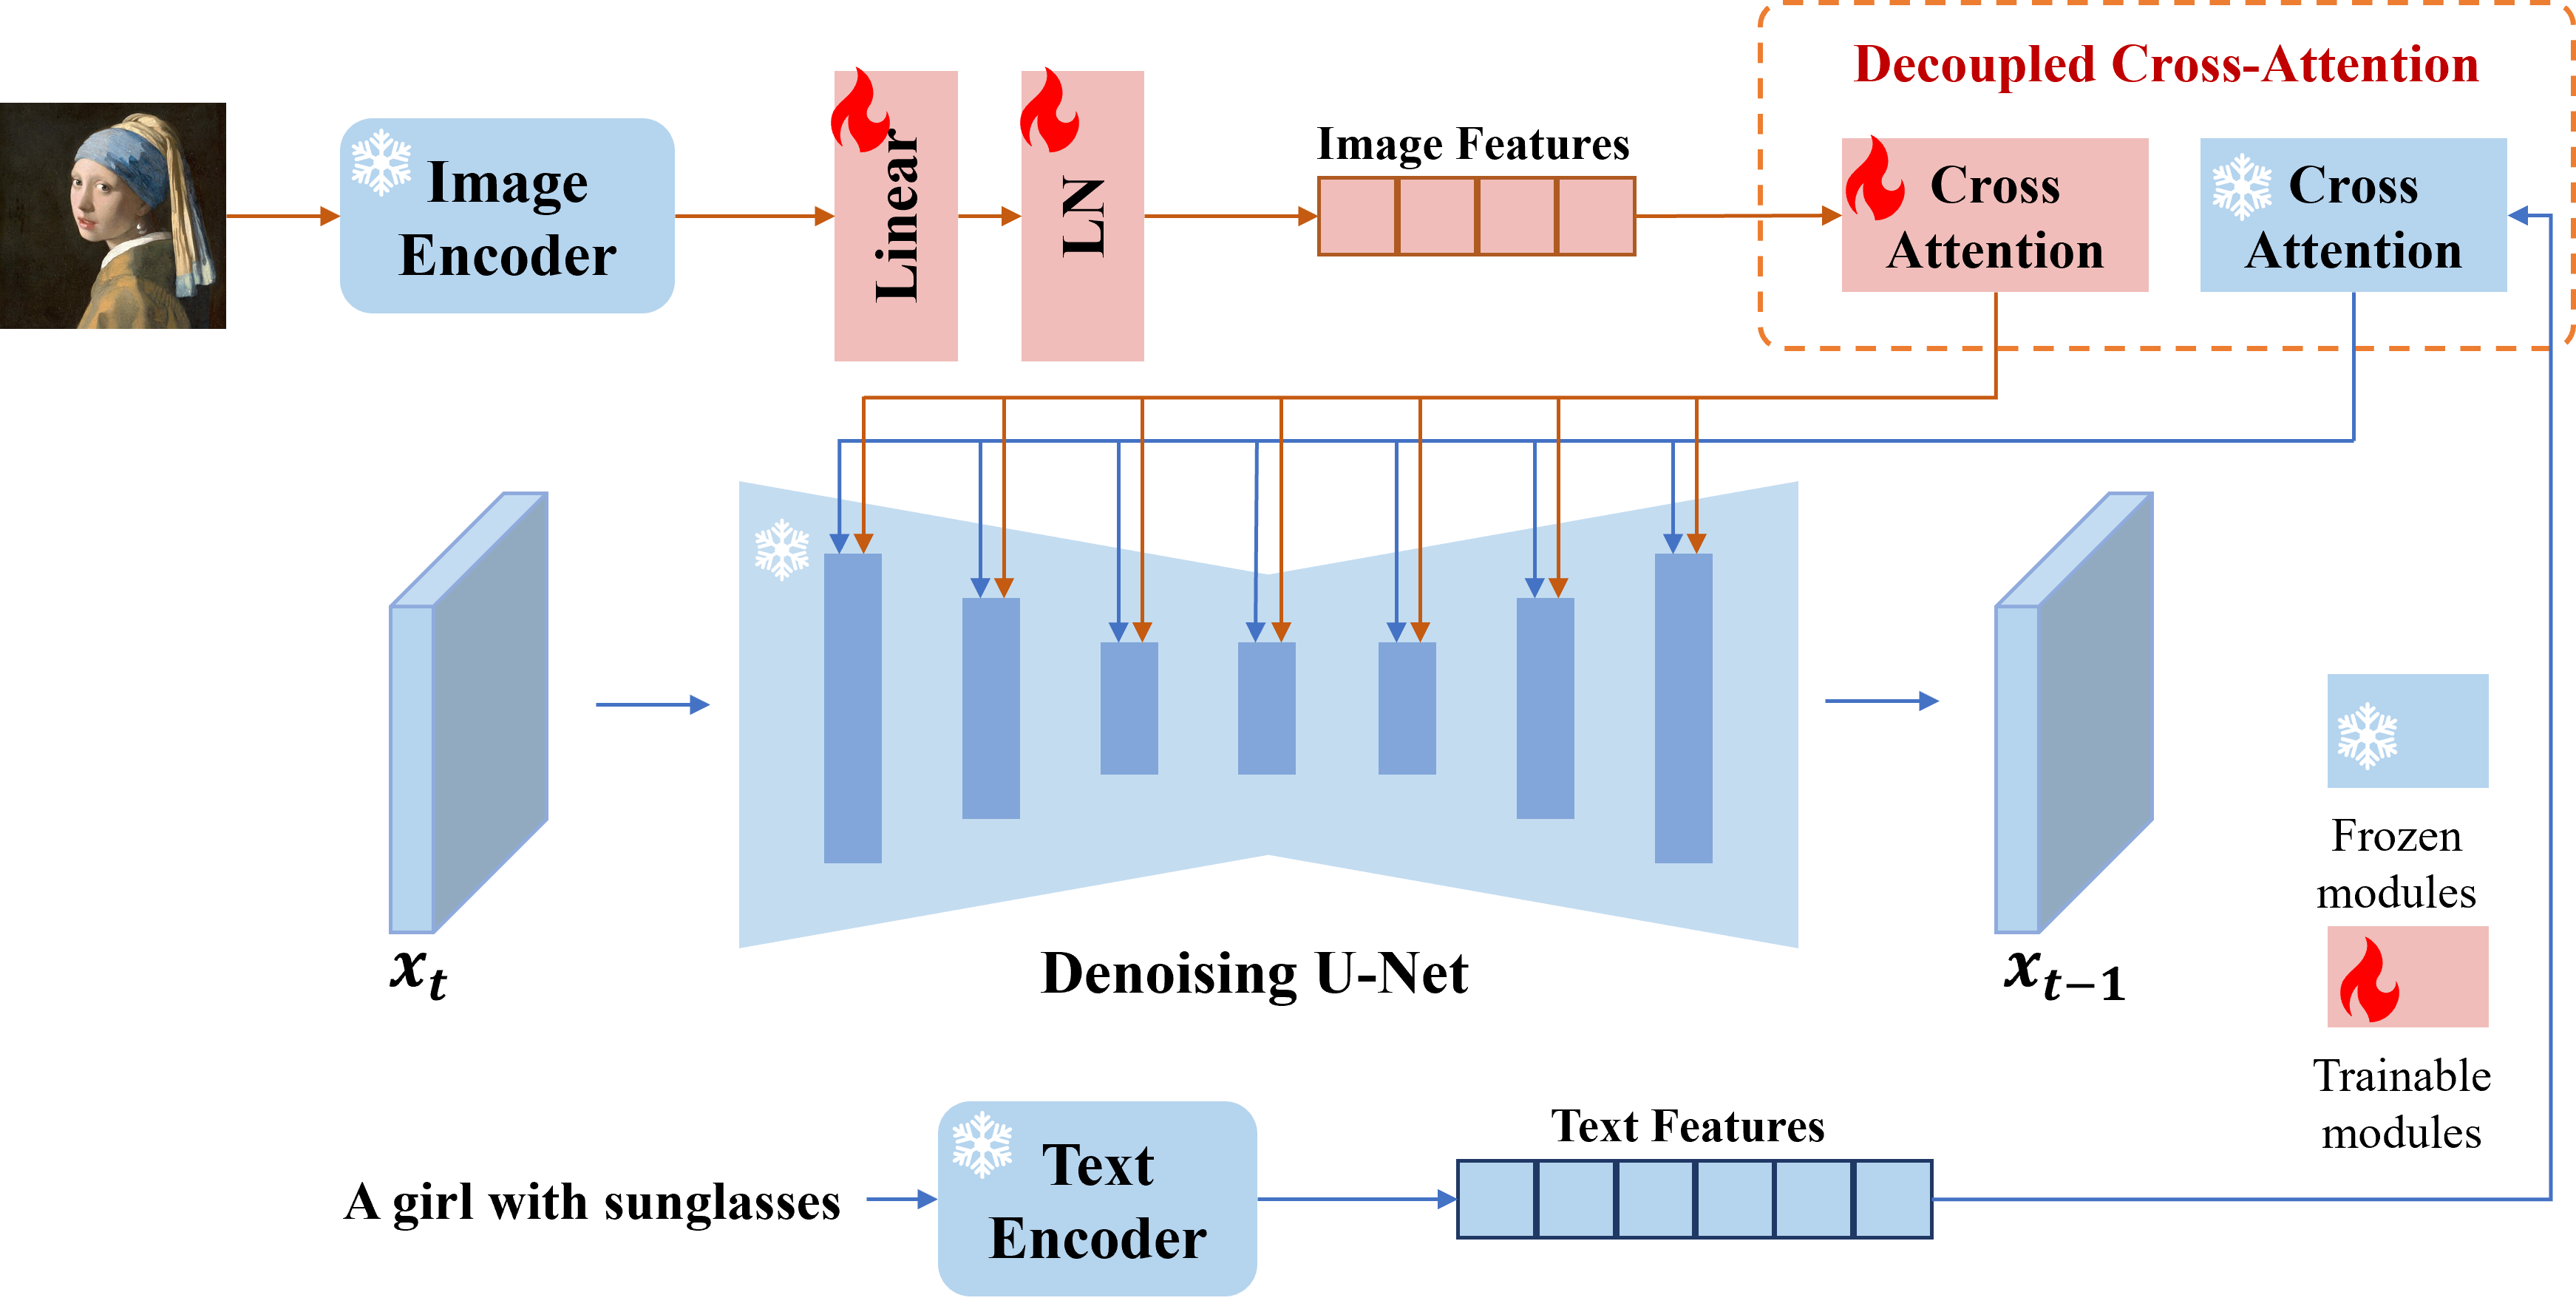
\includegraphics[width=0.7\textwidth]{images/related-work/ipadapter.png}
  \caption{Conceptual illustration of the IP-Adapter architecture, showing how image features extracted by an image encoder are integrated into the U-Net via dedicated cross-attention layers to guide the generation process. (Image based on the IP-Adapter concept)}
  \label{fig:ipadapter-concept}
\end{figure}

\subsubsection{CatVTON and UNet Feature Conditioning}
A particularly relevant approach for image conditioning, especially for tasks requiring detailed transfer of appearance or garment characteristics, is found in methods like CatVTON \cite{catvton}. The key insight in such methods is to leverage the rich, hierarchical features learned by the denoising U-Net itself. When provided with a reference image (e.g., an image of a specific garment), features can be extracted from various layers of the U-Net as it processes this reference. These extracted features, which encode information about texture, shape, and style at multiple scales, are then used to condition the generation of a new image (e.g., the same garment, but worn by a person). This conditioning can be achieved by injecting these features into the corresponding layers of the U-Net during the denoising process of the target image, often using attention mechanisms or direct feature fusion. This technique allows for a powerful form of image-based control that is highly attuned to the diffusion model's internal representations, facilitating tasks like virtual try-on with impressive fidelity by directly utilizing the U-Net's understanding of visual elements.

\subsection{Modulating Network Activations}
Feature-wise Linear Modulation (FiLM) \cite{film} is a general and effective technique for conditioning neural network activations. Instead of directly concatenating conditioning information or using complex gating mechanisms, FiLM applies a simple affine transformation to feature maps based on a conditioning input. Given a feature map $h$ from a layer in a neural network, and a conditioning vector $c$, a FiLM generator (typically a small neural network) produces a scale parameter $\gamma$ and a shift parameter $\beta$ from $c$. These parameters then modulate $h$ as follows: $FiLM(h) = \gamma \cdot h + \beta$. This allows the conditioning information $c$ to dynamically influence the behavior of the network layer by layer. FiLM is lightweight and can be integrated into various architectures to allow secondary inputs to control the processing of a primary input. Figure \ref{fig:film-layer} illustrates the internals of a FiLM layer.

\begin{figure}[h]
  \centering
  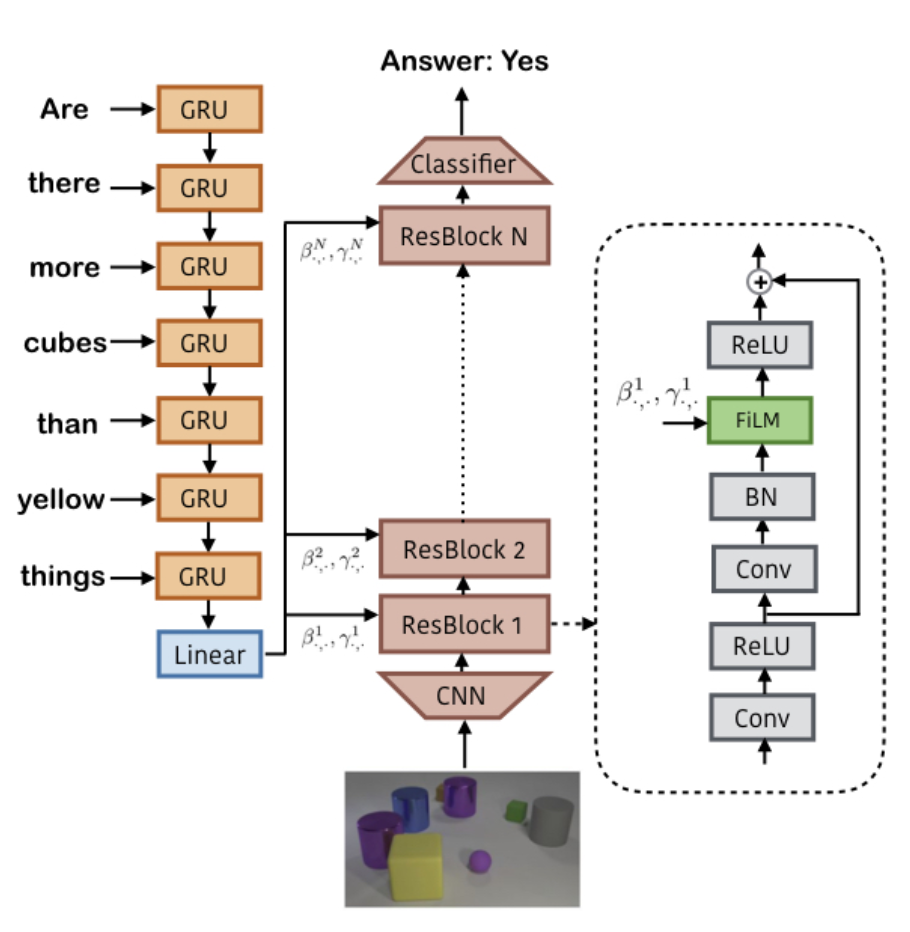
\includegraphics[width=0.5\textwidth]{images/related-work/film.png}
  \caption{The Feature-wise Linear Modulation (FiLM) layer. A conditioning input is processed by a FiLM generator to produce scale ($\gamma$) and shift ($\beta$) parameters, which then modulate the feature maps ($h$) of a main network. (Adapted from Perez et al. \cite{film})}
  \label{fig:film-layer}
\end{figure}

This approach enabled image-based models to effectively integrate and act upon conditioning information from outside the image domain. For instance, by modulating visual features based on encoded text tokens, it empowered (at the time) state-of-the-art image question answering models to ground their visual processing in textual context.

\subsubsection{FiLMed-UNet}
The FiLM technique has also been effectively applied to U-Net architectures in the medical imaging domain, notably in the FiLMed-UNet paper by Lemay et al. \cite{filmedunet}. Their work focused on enhancing medical image segmentation by incorporating various forms of metadata as conditioning signals. FiLMed-UNet utilized patient-specific information, such as tumor type or the target organ for segmentation.

The core idea was to make the U-Net's segmentation process adaptable and more informed by this external metadata. The metadata (e.g., one-hot encoded tumor type) was passed through a FiLM generator network, which produced scale ($\gamma$) and shift ($\beta$) parameters. These parameters then modulated the feature maps at different layers within the U-Net. This allowed the network to tailor its feature extraction and segmentation logic based on the provided metadata. For example, knowing the tumor type allowed the model to leverage type-specific visual characteristics, leading to improved segmentation accuracy. Furthermore, by conditioning on the desired output class (e.g., "segment kidney"), FiLMed-UNet demonstrated robustness in multi-task learning scenarios, even with missing labels for some tasks in the training data, and showed improved performance with limited annotations. While this application of FiLM is distinct from encoding camera parameters for 3D-aware synthesis, it highlights the versatility of FiLM in allowing neural networks to integrate and utilize diverse conditioning information to adapt their behavior for specialized tasks. Figure \ref{fig:filmed-unet-concept} shows a conceptual diagram.

\begin{figure}[h]
  \centering
  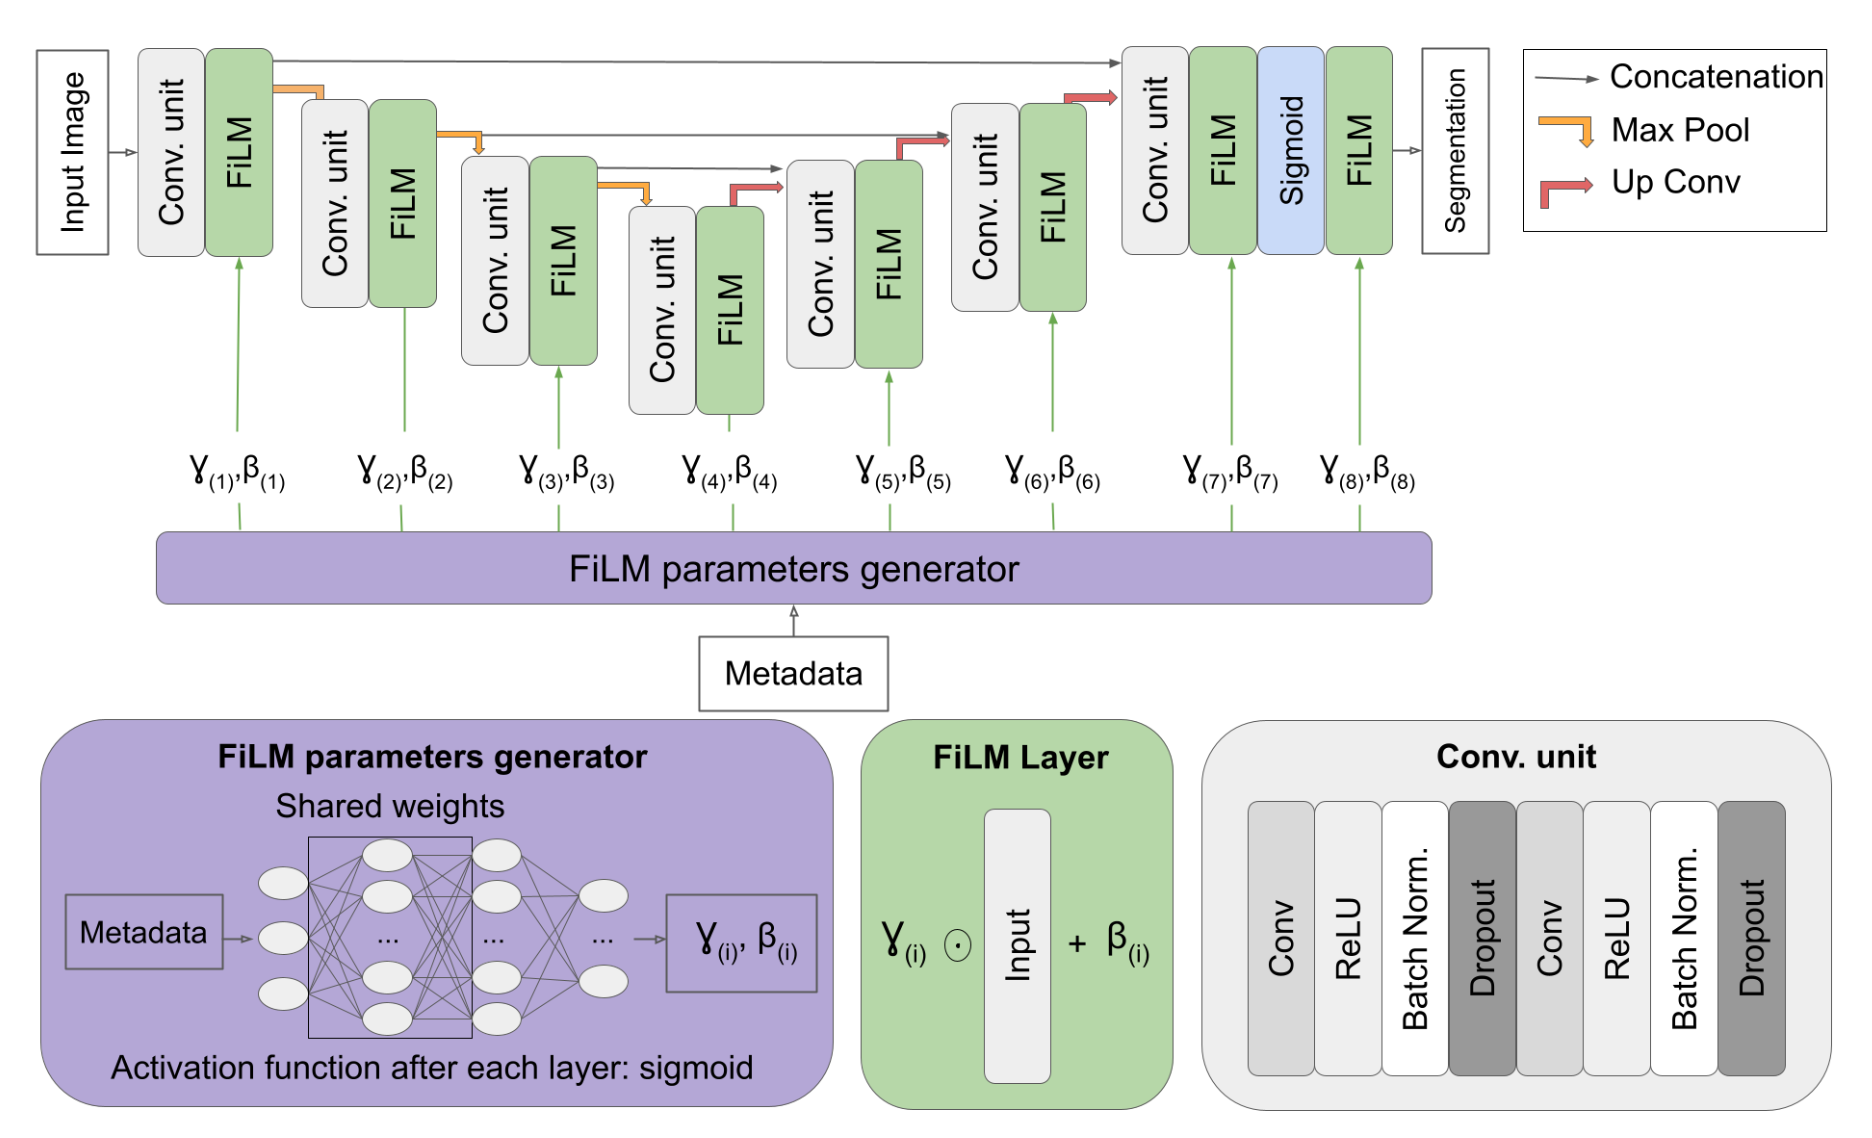
\includegraphics[width=0.7\textwidth]{images/related-work/filmed-unet.png}
  \caption{Conceptual diagram of a FiLMed-UNet. The metadata about patients are processed by a FiLM generator network, which outputs scale and shift parameters to modulate activations at various layers within the U-Net architecture, making the denoising process viewpoint-aware.}
  \label{fig:filmed-unet-concept}

\end{figure}

\subsection{Camera Parameter Encoding for 3D Awareness}\label{ssec:camera_param_encoding}
Making 2D diffusion models inherently 3D-aware is crucial for tasks like multi-view image generation. A key aspect of this is encoding camera parameters (Rotation R, Translation t) to guide the image generation process. Various methods focus on integrating this geometric information directly into the model's input or intermediate representations.

\subsubsection{Pixel-Level Geometric Conditioning: Ray-based Approaches}
This category of methods aims to provide detailed, per-pixel geometric information derived from camera parameters directly to the diffusion model.
A prominent technique is the use of a \textit{raymap}, as demonstrated by Watson et al. \cite{novelviewsynthesisdiffusion} in 3DiM and also utilized in CAT3D \cite{cat3d}. The raymap is a tensor with the same spatial dimensions as the image or latent representation. At each (u,v) coordinate, it stores the 3D origin and 3D direction of the camera ray passing through that pixel. In CAT3D, these rays are computed relative to the camera pose of the first conditional image.
To help the network learn high-frequency details associated with viewpoint changes, these ray origins and directions are often further processed using positional encodings.
The resulting positionally encoded raymap can be concatenated as an additional input channel to the U-Net, alongside the noisy image or latent representation \cite{novelviewsynthesisdiffusion, cat3d}. This allows the model to learn a direct, spatially varying mapping from ray geometry to the target pixel output.
% CAT3D \cite{cat3d} notes that such raymap conditioning generalizes better than using low-dimensional vector embeddings for camera pose, particularly for out-of-domain samples.

\subsubsection{Global Camera Pose Conditioning}
Alongside per-pixel data, global camera pose conditioning methods provide a more compact, holistic representation of the camera's viewpoint or transformation.
One approach involves \textit{vectorized transformation embeddings}. For instance, Zero-1-to-3 \cite{zero1to3} encodes the relative camera viewpoint transformation \(T = [R|t]\) between an input view and a target view as a 4x4 matrix. This matrix is flattened into a 16-dimensional vector, which is then projected by a small Multi-Layer Perceptron (MLP) and added to the timestep embedding. This globally influences the diffusion process by providing context about the desired viewpoint change.
Another technique employs \textit{decomposed pose vectors for attention mechanisms}. MV-Adapter \cite{mvadapter} represents each camera view using a 12-dimensional vector, which includes 3D camera coordinates and a 9D flattened rotation matrix. These vectors are processed by an MLP and then fed into multi-view attention layers as key and value components. This allows the model to explicitly attend to pose information when correlating features across different views, aiding in the generation of coherent multi-view imagery.

\section{Diffusion-based Multi-View Image Generation}\label{sec:multi-view-diffusion}

Building upon the camera parameter encoding techniques discussed in Section \ref{ssec:camera_param_encoding}, this section delves into specific diffusion-based models and architectures designed for generating single or multiple consistent views of a 3D scene or objects. These methods aim to leverage the generative power of diffusion models to synthesize novel perspectives, often with the goal of creating coherent 3D representations.

\subsection{Single Reference Image Novel View Synthesis}
Novel View Synthesis (NVS) from a single reference image is a challenging task that several diffusion-based approaches have tackled.

Zero-1-to-3 \cite{zero1to3}, an early pioneer in this area, conditions a latent diffusion model on a single reference image and a relative camera pose transformation \(T=[R|t]\) to generate a novel view. This model is fine-tuned from a pre-trained text-to-image model (Stable Diffusion). While demonstrating the potential for NVS without explicit 3D reconstruction, approaches like Zero-1-to-3 can sometimes face challenges in maintaining strong geometric consistency across widely varying generated views, a point often highlighted by subsequent multi-view generation methods \cite{imagedream, cat3d}.

Concurrently, Watson et al. \cite{novelviewsynthesisdiffusion} proposed 3DiM, a diffusion model designed for NVS that operates in pixel space. It conditions on a single source RGB-D image (though it can function with RGB only) and an absolute target camera pose. 3DiM utilizes the raymap technique for camera conditioning, as detailed in Section \ref{ssec:camera_param_encoding}, by constructing a raymap containing per-pixel 3D origin and direction, which is then positionally encoded and concatenated with the input image to the U-Net \cite{novelviewsynthesisdiffusion}. The model is trained to predict the clean target image from a noised source image.

\subsection{Coherent Multi-View Generation Architectures}
To improve consistency and enable robust 3D asset creation, several architectures focus on jointly generating or reasoning about multiple views simultaneously.

MVDream, often cited as a foundational multi-view model \cite{imagedream, mvadapter, cat3d}, extends diffusion models to generate multiple (e.g., four orthogonal) views from a shared text prompt by incorporating multi-view attention mechanisms. It learns from both 2D images and 3D assets to enhance 3D consistency \cite{mvadapter}.

Building on such concepts, ImageDream \cite{imagedream} introduces an image-prompt multi-view diffusion model. It takes a single image prompt and aims to generate multiple consistent views of an object. ImageDream leverages the canonical camera coordination (discussed in Section \ref{ssec:camera_param_encoding}) established by MVDream, where a default camera view corresponds to the object's front view. Its key architectural contribution is a multi-level image-prompt controller that integrates image features at global (CLIP global embedding), local (CLIP hidden features), and pixel (VAE encoded image latent) levels into the MVDream-like diffusion U-Net \cite{imagedream}. The pixel controller, for instance, concatenates the input image prompt's latent as an additional frame to the four target views, enabling 3D self-attention across all five frames. ImageDream employs Multi-View Score Distillation Sampling (MV-SDS) for reconstructing a NeRF from the generated views.

CAT3D \cite{cat3d} presents a multi-view diffusion model designed to simulate a real-world capture process by generating a large set of consistent novel views from one or more input images and specified target camera poses. Its architecture is similar to video latent diffusion models \cite{stablevideodiffusion}, employing 3D self-attention (2D in space and 1D corresponding to time across images) and is initialized from a pre-trained latent diffusion model. For camera conditioning, CAT3D uses the raymap approach (see Section \ref{ssec:camera_param_encoding}), where ray origins and directions are computed relative to the first conditional image's camera pose and concatenated channel-wise to the latents \cite{cat3d}. To generate a large number of views (e.g., 80 for single-image input, up to 960 for few-view), CAT3D can group target viewpoints and, for single-image inputs, may first autoregressively sample a set of anchor views before generating the remaining views. These generated views are then used as input to a robust 3D reconstruction pipeline (e.g., Zip-NeRF).

ViewCrafter \cite{viewcrafter}, as noted by CAT3D \cite{cat3d}, combines video latent diffusion models with 3D point cloud priors. This approach aims to achieve high-fidelity and consistent novel views by leveraging explicit 3D information alongside the generative capabilities of video diffusion models, enabling precise camera control.

While these architectures show impressive results, methods requiring full fine-tuning of large pre-trained models are expensive and may risk performance degradation if high-quality, large-scale 3D data for fine-tuning is scarce.

\subsection{Specialized Multi-View Adapters}
To mitigate the challenges of full fine-tuning, adapter-based methods offer a lightweight alternative for enabling pre-trained models with multi-view generation capabilities.

MV-Adapter \cite{mvadapter} is a notable example, introducing a plug-and-play adapter for multi-view image generation that enhances pre-trained text-to-image diffusion models while preserving their original network structure and feature space. It employs a decoupled attention mechanism: the original spatial self-attention layers of the pre-trained model are kept frozen, and new multi-view attention layers are created by duplicating the structure and weights of these original layers. These new layers, organized in a parallel architecture, process features from multiple views (typically packed along the batch dimension) and learn geometric knowledge efficiently \cite{mvadapter}. 

For encoding geometric information, MV-Adapter \cite{mvadapter} integrates camera parameters using raymaps, an approach also seen in methods like 3DiM \cite{novelviewsynthesisdiffusion} and CAT3D \cite{cat3d}. These raymaps can be positionally encoded and are then typically supplied as additional input channels to the U-Net, processed by the adapter's components. This method of providing direct geometric cues, combined with other conditioning signals like text or image embeddings processed through its attention mechanisms, allows for flexible control in tasks such as text-to-3D and image-to-3D generation. By updating significantly fewer parameters than full fine-tuning—primarily those of the adapter module—MV-Adapter enables efficient training, preserves the rich priors of the base model, and reduces the risk of overfitting.